% Chapter Template
\chapter{Related Work} % Main chapter title

\label{chapter::related_work} % Change X to a consecutive number; for referencing this chapter elsewhere, use \ref{ChapterX}

\lhead{Chapter 2. \emph{Related Work}} 

In this chapter, we provide a review of state-of-the-art tracking methods.
Numerous approaches for object tracking have been proposed before. These methods
differ from each other based on the way the authors solve common questions, such
as: Which object representation is suitable for tracking the target? How can
motion, appearance, or shape of the object needs to be modeled?. The answers 
for these questions depend on the context/environment where tracking is
performed and the visual features of the object that needs to be tracked. This
chapter is focused on presenting methodologies for object tracking in general
and not for specific objects, such as humans or faces.

We follow a structure for describing the issues that are necessary to address,
when building an object tracker. In section \ref{sec::object_representation} we
describe common object representations and image features. Section
\ref{sec::detection} summarizes general schemes for detecting objects in an
scenario. In Section \ref{sec::tracking}, we categorize and describe
existing tracking methods. Section \ref{sec::datasets} shows existing
datasets used for object tracking and explains challenges which are present
in different video sequences. Finally, we show in Section \ref{sec::ensemble}
recent tracking methods that perform ensemble of multiple trackers or features.

\section{Object representation and visual features.}
\label{sec::object_representation}

An object can be considered simply as nothing but an entity of interest used for
further analysis. For instance, birds in the sky, pedestrians, vehicles on a
road, ships on the sea, are set of objects necessary to track in a specific
context. These elements can be represented by their shape or appearance.
According to the object that is chosen to be tracked, an object representation
is selected instead of the rest. For tracking small objects
in a scenario, point representation is usually appropiate
\cite{Veenman2001,Shafique2005}. In the case of tracking objects whose shapes
are approximated to rectangle and ellipses, shape representation is more
appropiate \cite{Comaniciu2003a}. To track objects with complex shapes, such
as humans or excavators machines, contour or silhouette-based representation are
appropiate \cite{Haritaoglu2000}.

In order to track objects, selecting the right features plays a critical role.
In general, a \gls{feature} is a property of an image which we are interested in.
The most important property of a visual feature is its uniqueness so
that could be easily distinguished from other objects. Mostly features are
chosen manually by the user depending on the application domain. This problem of
automatic feature selection has received significant attention in the pattern
recognition community. The most common visual features selections are color
\cite{Paschos2001,Song1996}, edges \cite{Canny1986,Bowyer2001}, displacement
vectors \cite{Black1996,Lucas1981a}, corners \cite{Harris1988} and textures
\cite{Haralick1973,Nickels1997,Mallat1989}.Among all features, color is one
of the most widely used feature for
tracking. However, color features are sensitive to illumination variation. To
tackle this problem, in scenarios where this effect is inevitable, other
features are incorporated to model the appearance of an object.

\section{Moving Object Detection} 
\label{sec::detection}

Every tracking approach requires an object detection approach as
initialization, or in every frame of the video. Detection can be defined as
finding instances of objects in images or videos. A common method for object
tracking is to apply object detection when the object appears for the first
time, reducing the number of false detections. 

A large number of methodologies have been proposed for object tracking, focusing
on the task of object detection first. Most of them apply combinations among
different methodologies, making it very difficult to create a uniform
classification of existing approaches. This section classifies
different approaches available for object detection from videos.

\subsection{Background Subtraction}

Background subtraction is a commonly used technique for object segmentation in
static scenarios \cite{McIvor2000}. This task consists in detecting moving
regions by subtracting the current image pixel-by-pixel from a reference
background image. The pixels above some threshold are classified as foreground
(belongs to an object). The background image is created averaging images over
time in an initialization period, and is updated with new images to adapt to
dynamic scene changes. Also, the foreground map is followed by morphological
operations such as closing and erosion (elimination of small-sized blobs).

Although background subtraction techniques extracts well most of the relevant
pixels, this method is sensitive to changes when some background and foreground
pixels have similar value.

\begin{figure}[h!]
	\centering
		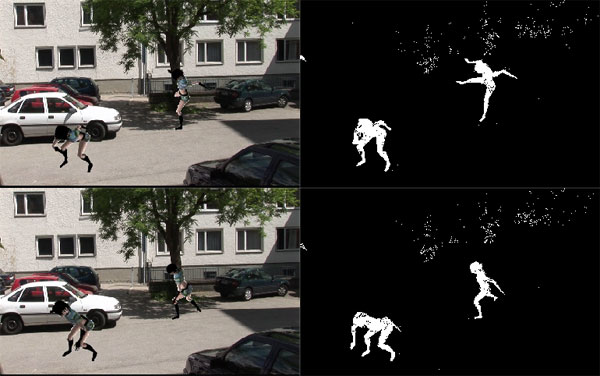
\includegraphics[width=0.7\linewidth]{Figures/bg_sub.jpg}
	\caption[Object detection using Gaussian Mixture Models for background
	subtraction]
	{Object detection using Gaussian Mixture Models for background
	subtraction. Foreground pixels are drawn in white. Figure reproduced from
	\cite{Pham2010}}
	\label{fig::bg_sub}
\end{figure}

\subsection{Temporal differencing}

In temporal differencing, objects are detected by taking pixel-by-pixel
difference of consecutive frames (generally two or three) in a video sequence.
This method is most common for object detection in scenarios where camera
is moving. Unlike static camera scenarios, the background is changing rapidly
(not appropiate to create a background model). Alternatively,
the moving object is detected by taking the difference between frames $t - 1$
and $t$.

This method is highly adaptive to dynamic changes in the scene as most recent
frames are involved in the process. However, it fails detecting new small
regions as moving objects (ghost regions). Detection will not be correct either,
for objects that preserve uniform regions (static objects).

A two-frame differencing method is presented in \cite{Lipton1998a}, where the
pixels that satisfy the following equation are marked as foreground.\\
\centerline{$|I_t(x,y), I_{t-1}(x,y)|>Th$}

Other methods were developed in order to overcome drastic changes of two frame
differencing. For instance, a three-frame differencing method \cite{Wang2003} 
and a hybrid method which combines three-frame differencing with an adaptive
background subtraction model \cite{Collins2000}.

\subsection{Statistical Approaches}

Statistical characteristics of pixels have been used, in order to overcome
shortcomings between frames of basic background subtraction methods. The
approaches consist in keeping and updating pixels statistics that belong to the
background model. Foreground pixels are identified by comparing each pixel's
statistics with that of the background model. These methods are becoming more
popular due to its reliability in scenes that contain noise, illumination
changes and shadows. Some approaches apply Hidden Markov Models (HMM). These
methods \cite{Stenger2001,Rittscher2000} represent the intensity variation of a
pixel in an image sequence as discrete states

The statistical method proposed in \cite{Pham2010} describes and adaptive
background model for real-time tracking. Every pixel is modeled by a mixture of
Gaussians which are udpated online using incoming image data. Then, the
Gaussians distributions of the mixture model for each pixel is evaluated
in order to detect whether a pixel belongs to foreground and background.

\subsection{Point detectors}

Point detectors are used to find interesting points in objects which have an
expressive texture in their respective localities. An interest point should
have invariance to changes in illumination and camera viewpoint. One important
detector uses optical flow (KLT) approach \cite{Shi1994}. This method make use
of the flow vectors of moving objects over time to detect moving blobs in an
image. In this approach the apparent velocity and direction of every pixel in
the frame must be computed. Some other methods are SIFT \cite{Lowe2004b} and
Harris \cite{Harris1988} corners detectors.

\begin{figure}[h!!]
\centering
{
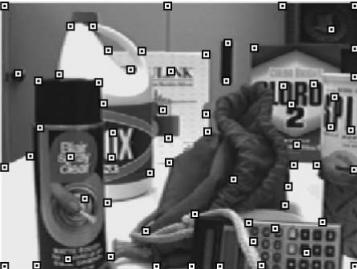
\includegraphics[width=0.32\linewidth]{Figures/points/harris.png}
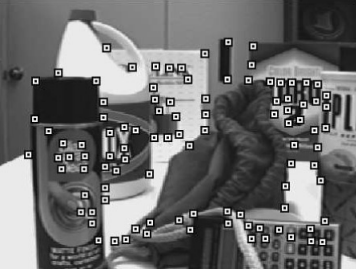
\includegraphics[width=0.32\linewidth]{Figures/points/klt.png}
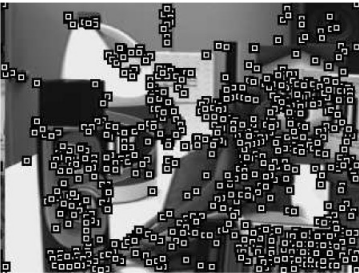
\includegraphics[width=0.32\linewidth]{Figures/points/sift.png}
}	
\caption[Interest points for object detection]
		{Interest points for object detection. Left - Harris, center - KLT, 
		right - SIFT. Figure reproduced from \cite{Yilmaz2006}.}
\end{figure}

\section{Object Tracking}
\label{sec::tracking}

The goal of an object tracker is to generate an object trajectory in a video.
This path consists of the object position across the time. Additionally,
a tracker may provides other information, such as scale, orientation, area, or
shape of an object. This section classifies ans covers popular approaches
for object tracking on each category.

\subsection{Point Tracking}

Tracking can be formulated as the correspondence of objects represented by
points across frames. This category can be divided into two subcategories:

\textbf{Deterministic Methods. } These approaches for point correspondence
define a cost of associating each object in frame $t-1$ to a single object in
frame $t$ using motion constraints, such as proximity, velocity, rigidity and
motion. Minimization of the correspondence cost is formulated as a
combinatorial optimization problem. A solution, which consists in one-to-one
correspondence among all possible associations, can be obtained by optimal
assignment methods. For instance Hungarian Algorithm \cite{Qin2012} or
greedy search methods.

\textbf{Statistical methods for Point Tracking. } Statistical correspondence
methods solve tracking problems whose measurements obtained from video sensors
contain noise, or object motion can undergo random perturbations. These
approaches take measurements and model uncertainties into account during
object state estimation. Applying state space approach to modeling the object
properties such as position, velocity and acceleration. In single object
state estimation, the optimal state of an object is given by a Kalman Filter
\cite{Ren2008a,Heikkila2004}, assuming measurement noise have a Gaussian
distribution. In the general case, that is, object state is not assumed as
Gaussian, estimation can be performed using particle filters
\cite{Okuma2004,Rittscher2000}.

In the case of multiobject data association, it is necessary to solve first
correspondence problem before these filters can be applied. However, in cases
when two objects are close each other, the correspondence could be incorrect.
Then, an incorrectly associated measurement can cause the filter to fail to
converge. In order to tackle this problem, Joint Probability Data Association
Filtering (JPDAF) \cite{Schulz2003} and Multiple Hypothesis Tracking
(MHT) \cite{Zulkifley2012} are two used techniques for data association.

\begin{figure}[t!!]
\centering
{
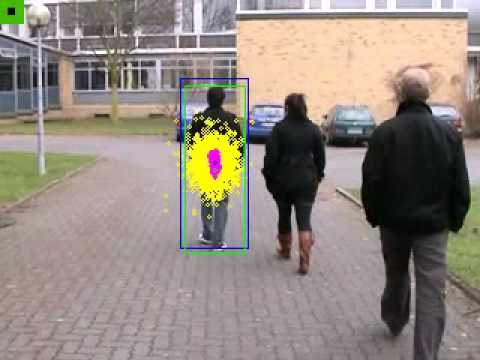
\includegraphics[width=0.32\linewidth]{Figures/particle_filter1.jpg}
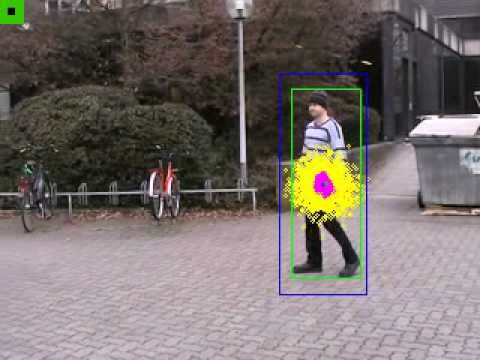
\includegraphics[width=0.32\linewidth]{Figures/particle_filter2.jpg}
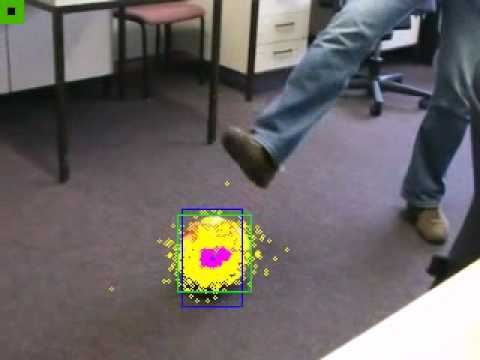
\includegraphics[width=0.32\linewidth]{Figures/particle_filter3.jpg}
}
\caption[Object tracking using particle filter]
		{Object tracking using particle filter. Each particle represents one
		possible location of the object being tracked. A set of particles have
		more weight at locations where is more likely to be the object. Figure
		reproduced from \cite{Rittscher2000}}
\end{figure}


\subsection{Kernel Tracking}

In this type of tracking, the object motion is computed using representations
of a primitive object region, from one frame to the next. These algorithms
differ in terms of appearance representation, the number of objects to be
tracked, and the method used for object motion estimation. 

\textbf{Density-based tracking:} According to \cite{Cheng1995}, the object is
modeled with one or more probability density functions, such as
Gaussian, mixture of Gaussian, Parzen windows or histograms, that describe
the probability of object appearance. Mean-shift is an approach of density-based
tracking. This method shifts a data point to the average of data points
in its neighborhood, using fixed color distribution. A similar
approach is called CAMSHIFT \cite{Exner2010} that handles dynamically
changing color distribution by adapting the search window size
and computing color distribution in the search window.

\textbf{Template-based tracking:}  These approaches apply templates of the
object to calculate appearance probability on every frame of the
video sequence. The most common is \textit{Template \gls{matching}} \cite{Korman2013}
that searchs accross the image, a region similar to the object template, defined
in previous frames. The similarity measure is calculated using normalized cross
correlation. A limitation of this method is its high computational cost due to
brute force search. To reduce this cost, some methods limit the object search
to a neighborhood near previous position.

Instead of templates, other object representations can be used for tracking.
For example, color histograms or mixture models can be computed using the
appearance of pixels inside a rectangular or ellipsoidal region. To reduce
computational complexity, the similarity between object model and the
hypothesized position, is computed evaluating the ratio between color means of
object model and position. The position with highest ratio is selected as
current object location.

\begin{figure}[t]
	\centering
		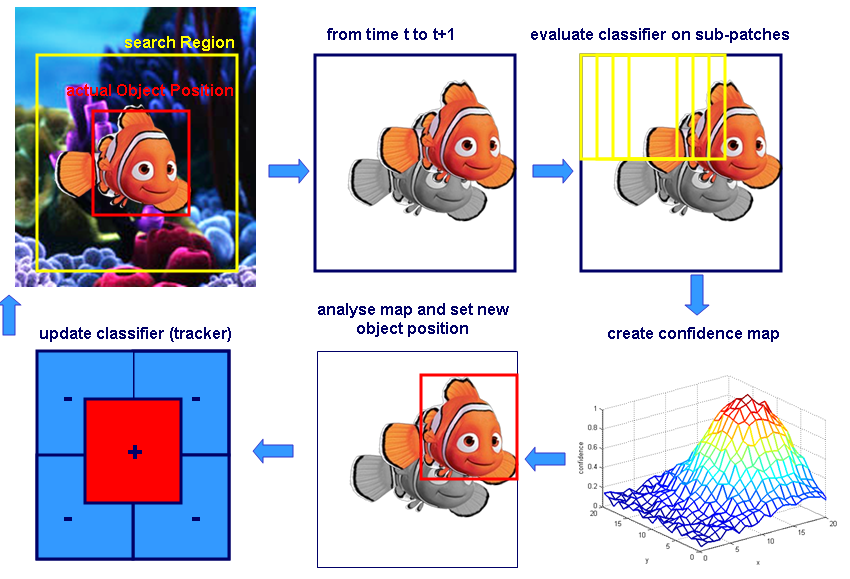
\includegraphics[width=0.7\linewidth]{Figures/overview_boost.png}
	\caption[Overview for online boosting object tracker]
	{Overview for online boosting object tracker. For each classified patch,
	the system receives a confidence value, that is entered into a 
	confidence map. Using the confidence map, the tracking windows is
	shifted to the best possible position. Then, the classifier is updated and
	the	process is repeated. Figure reproduced from \cite{Grabner2006}}
	\label{fig::overview_boost}
\end{figure}	

"Tracking by detection" \cite{Mori2006} systems generally perform target object
appearance learning. These methods are closely related to object detection
(an area with great progress in computer vision) and has encouraged some
successful real-time tracking algorithms \cite{Liu2007,Grabner2006}. However,
many tracking algorithms employ static appearance models that are defined
manually or trained at the first frame only \cite{Isard2001, Lepetit2006,
Black1996, Comaniciu2000, Adam2006}, these methods are often unable to deal
with significant appearance changes. In order to cope this problem, an adaptive
appearance model that changes during the tracking process as the appearance of
the object changes, gets better results \cite{Ross2007,Matthews2004,Jepson2003}.

Boosting has been used in a wide field of machine learning tasks and
applied to computer vision problems. Many tracking algorithms are based on the
boosting framework \cite{Freund1997a} and is related to the work on
Online Adaboost \cite{Avidan2007,Grabner2008,Oza2000}, multi-class boost
\cite{Saffari2010} and MILBoost \cite{Babenko2010}. The goal of boosting is
to combine many weak classifiers (usually decision stumps) into a linear
strong classifier.

\textbf{Sparse/non.sparse representation: } In this type of tracking, a set of
target samples is associated with spanned serveral templates. The likelihood
of a candidate sample belonging to the object class is often determined by the
residual between the candidate sample and the reconstructed samples derived from
a linear representation \cite{Zhang2012b,Zhang2012a,Bao2012,Mei2011a,Mei2011}.

\subsection{Silhouette Tracking}

The object is tracked via estimation of the object region in each frame.
Silhouette-based methods provide an accurate shape description for the
objects that are tracked. These approaches can be divided into two main
categories, shape matching and contour tracking. Shape matching \cite{Li2001}
approaches search object silhouette in the current frame. Contour based, evolve
initial contour to its new position using state space models or direct
minimization of an energy function \cite{Cremers2003}.

\begin{figure}[h!]
	\centering
		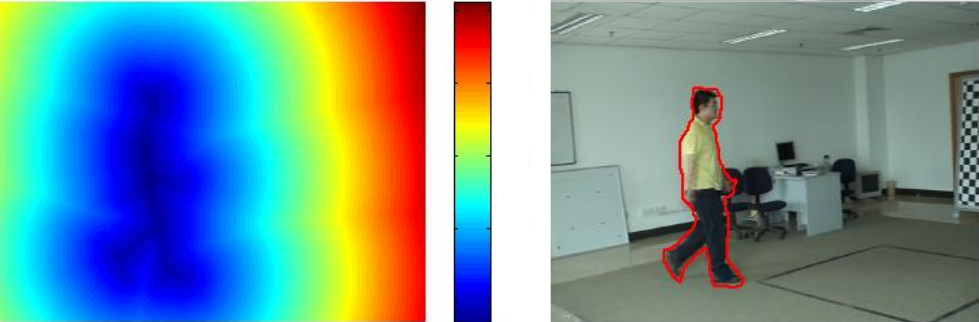
\includegraphics[width=0.9\linewidth]{Figures/contour.png}
	\caption[Illustration of an active contour representation]
			{Illustration of an active contour representation. Left subfigure
			shows the signed distance map of a human contour; right
			image displays contour result. Figure reproduced from \cite{Yilmaz2006}}
	\label{fig::contour}
\end{figure}	
\section{Tracking Datasets and Challenges}
\label{sec::datasets}

\textbf{Tracking Challenges. }Object detection and tracking is still an open
research problem in computer
vision. A robust, accurate and high performance approach is still a great
challenge. The level of difficulty depends on how the object of interest is
defined in terms of features. For instance, Using color as object representation
method, it is not difficult to identify all pixels with same color as the
object. However, there is always a probability of existence a background region
with same color information (background clutter). In addition, illumination
changes in the scene does not guarantee that the pixel values of an object
will be the same in all frames. These variabilities or challenges which are
random in object tracking causes failures, and are listed below.

\begin{itemize}
\item \textbf{Illumination Variation (IV):} It is desirable that background
model adapts to gradual changes of the appearance of the environment.
\item \textbf{Scale Variation (SV):} Ratio between initial object size and
current object size differs.
\item \textbf{Occlusion (OC):} Partially or full, occlusion affects the process
of computing the background frame. In real life situations, occlusion can occur
anytime the object of interest passes behind another object with respect to a
camera.
\item \textbf{Dynamic background:} Some scenery regions contain movement, but
should be still remain as background, acoording to their relevance. Such
movement can be periodical or irregular, causing blurring (motion blur - MB),
e.g. traffic lights, waving trees).
\item \textbf{Out of view (OV): } Some portion o the target leaves the view.
\item \textbf{Background clutter (BC):} As stated before, this challenge makes
the segmentation task difficult. It is hard to create ans separate background
model from moving foreground objects.
\item \textbf{Fast Motion (FM):} The speed of a moving object plays an
important role in its detection and track. If an object is moving too slow,
the temporal differencing methods fails to detect object, because it preserves
uniform region between frames. In the other case, fast moving object leaves
ghost regions in a detected foreground model.
\item \textbf{Object rotation and deformation (DEF):} Since natural objects
move freely, they can appear slightly or completely transformed. Such
rotations, in (IPR) or out (OPR) of plane on the images affect object tracking
considerably.
\item \textbf{Low Resolution (LR):} Number of pixels inside the object
bounding box is less than 400.
\end{itemize}

\textbf{Tracking Dataset. } In computer vision, a \textit{dataset} could be
defined as a collection of
images or video sequences used for testing algorithms. The amount of data and
characteristics presented, depend on the field that is studied.
For instance, in scene recognition, a dataset contains images of landscapes or
outdoor environments. Generally, this collection is shared between researchers
and plays an important role in comparison and evaluation of state-of-the-art
approaches. A list of datasets used in object tracking is summarized in table
\ref{table:datasets}

The Surveillance Performance Evaluation Initiative (SPEVI) \cite{Maggio2005}
can be used for evaluating algorithms for surveillance-related applications. The
first dataset contains 5 sequences applied to single person/face detection and
tracking. The second dataset applies for multiple person/face detection and
tracking. The sequences contain four targets occluding each other repeatedly.
ETISEO dataset \cite{Munder2006} contains indoor and outdoor scenes, such as
corridors, buildings entries, etc. This dataset can be used for surveillance
applications.

PETS dataset \cite{PETS} became a surveillance project whose challenging
scenarios are focused only on high level applications of this field. Some
issues, like illumination or scale changes are not considered in these videos.
Most of the sequences are used for person/vehicle tracking in outdoor
environments(subway stations, building entrances). CAVIAR \cite{Torralba2003}
is a dataset used generally for situation recognition systems. However,
sequences can be applied for tracking evaluation methods. Includes videos of
people walking alone, meeting other people, entering and exiting shops.

The VIdeo Surveillance Online Repository (VISOR) \cite{Vezzani2010} database
covers a wide range of scenarios and situations, including videos for human
action recognition, outdoor videos for face detection, indoor videos for people
tracking with occlusions, vehicles detection and surveillance. The VIdeo
Surveillance Online Repository, includes several sequences for two separate
tasks: First, an abandoned baggage scenario and second, a parked vehicle
scenario.

Recently, the tracking community released evaluation suites containing a
selection of videos and algorithms for testing trackers performance. These
benchmarks test and compare many tracking approaches using fair evaluation
criteria. Online Object Tracking Benchmark \cite{Wu2013B} contais 50 most
commonly used sequences. Also, the authors classified tracking challenges
(attributes) into subsets to report specific challenging conditions. The
Amsterdam Library of Ordinary Videos for tracking, ALOV300+ \cite{Smeulders2014},
consists in 315 real-life video sequences from Youtube with 64 different
targets. The collection is categorized for thirteen aspects of difficulty and
evaluates a large variety of situations including low contrast, occlusion,
ilumination variation, etc.

\begin{table}[t!]
\centering
\begin{tabular}{lccc}
\toprule
\textbf{Dataset} & \textbf{\# Sequences} & \textbf{GT-Available} &
\textbf{Object} \\ \midrule
Bobot \cite{KleinIROS10}          & 12       & Yes & Generic \\
Cehovin \cite{Cehovin2013}        & 5        & Yes & Generic \\
Kalal \cite{Kalal2011}            & 10       & Yes & Generic \\
Kwon \cite{KwonL09}               & 4        & Yes & Generic \\
Kwon VTD \cite{KwonL10}           & 11       & Yes & Generic \\
PROST \cite{Santner2010a}         & 4        & Yes & Generic \\
Ross \cite{Ross2007}              & 4        & Yes & Generic \\
Thang \cite{Dinh2011}             & 4        & Yes & Generic \\
Wang (NoRef)                      & 4        & Yes & Generic \\
Tracking Benchmark \cite{Wu2013B} & 50       & Yes & Generic \\
ALOV 300+ \cite{Smeulders2014}    & 315      & Yes & Generic \\
Godec \cite{godec11a}             & 7        & Yes & Human   \\
Babenko \cite{Babenko2010}        & 3        & Yes & Human   \\
SPEVI \cite{Maggio2005}           & 3,5      & Yes & Human   \\
ETISEO \cite{Munder2006}          & 86       & Yes & Human   \\
PETS \cite{PETS}                  & 23 		 & Yes & Human   \\
CAVIAR \cite{Torralba2003}        & 25   	 & Yes & Human   \\
Clemson \cite{Birchfield1998}     & 16       & Yes & Human   \\
VISOR \cite{Vezzani2010}          & 6        & No  & Human   \\
\bottomrule
\end{tabular}
\caption{Object tracking datasets.}
\label{table:datasets}
\end{table}

\section{Object tracking applying ensemble}
\label{sec::ensemble}

Several methods have proposed the use of ensemble classifiers within
the tracking-by-detection framework.
%The first algorithm that explicitly applies ensemble methods to
%tracking-by-detection is presented in \cite{Avidan2007}.
In this perspective, instead of ensembling the outputs of other trackers,
these methods focus on building ensemble classifiers,
such as Adaboost \cite{Avidan2007} or Bayesian probabilistic fusion \cite{Bai2013},
from weak low-level image features.
The classifier is then used to detect the target object in
new frames. Instead of working directly with low-level image features,
our ensemble tracker builds on top of tracker outputs
which are used as a more powerful mid-level representation of the target.
%Considering tracking as a binary classification problem, the author
%extends \cite{Collins2005} by using the Adaboost algorithm to
%combine a set of weak features and online updating of the object model.
%The classifier is then used to classify pixels in the next
%frames as either related to the object or background, which produces
%a confidence map of the location of the object.

Another alternative is to manually select a small set of trackers and use
prior knowledge on the behaviour of each tracker to build an ensemble.
In \cite{Santner2010a}, the authors combine a template-based tracker,
an optical flow tracker, and an online-random forest tracking-by-detection
method into a cascade.
In that case, the authors manually predefine a set of rules that decide
how to ensemble the tracker outputs. In contrast, our method can handle
a larger pool of trackers in the ensemble, since their outputs are combined
in a data-drive fashion that does not require manual rules or prior knowledge
on the behaviour of each tracker.
%The best selection is summarized into a simple
%set of rules. The authors explain that augmenting or updating in a smart way
%a simple online learner in terms of adaptivity can lead to much better results.


Sampling based approaches have also been explored for ensemble tracking.
Examples of this are the VTD \cite{Kwon2009} and
VTS \cite{Kwon2011a} trackers.
In this perspective, there is a sampling process that generates
multiple samples of target and tracker states. These trackers run in parallel
and their outputs are fused by probabilistic weighting. Therefore,
the ensemble uses a set of trackers of similiar architecture
with varying parameters. Our ensemble has the advantage of fusing outputs
of multiple trackers with no assumptions on their architectural similarity
and can leverage strenghts that different tracker architectures can provide.
%In these articles, the approaches obtain several samples of target and trackers
%states during sampling process using a Markov Chain Monte Carlo method.
%The trackers are sampled by proposing appearance models, motion models,
%state representation types, and observation types.
%Then, the sampled trackers run in parallel and interact with each other,
%covering target variations.

%The authors in \cite{Bai2013} proposed a classifier ensemble framework that
%uses Bayesian estimation theory to estimate the non-stationary distribution
%of sampled classifiers.
%In contrast with general tracking-by-detection classifiers,
%the weight vector that combines the classifiers is treated as a random
%variable and the posterior distribution of this vector is treated using
%Bayes' theory.
%Our approach presents a self-learning algorithm that enables
%object model updates based on tracking results and not from Bayesian updates of
%the classifier.

Finally, one can consider the case of offline fusion of trackers, such as in
\cite{Bailer2014}, where all trackers are applied to the entire sequence
and the ensemble is performed after the entire sequence is processed.
However, we are interested in the case of online tracking,
where the full sequence is not available beforehand. Furthermore, our online
approach is capable of steering and reinitializing failed trackers, increasing
the chances of better long-term tracking performance.

%the authors present an approach
%that merges the result of different tracking algorithms to produce a better
%tracking result.
%Based on the idea of attraction fields, which means the closer
%a fusion candidate is to a tracking result box,
%the stronger it is attracted by it.
%The result that maximizes the attraction of all trackers is chosen as a
%global result. In contrast, our fusion approach does not drop out bad tracking
%results. Our method is able to find and reinitialize outliers efficiently.

